\documentclass[tikz,border=4pt]{standalone}
\usepackage{tikz}
\usepackage{amsmath}
\usepackage{amssymb}
\usetikzlibrary{arrows.meta,positioning,fit,backgrounds,shapes.geometric,
                decorations.pathreplacing,calc,shadows.blur,shapes.arrows}

% ------------------------------------------------------------------
% Color palette (muted, print-safe, AAAI-friendly)
% ------------------------------------------------------------------
\definecolor{frozenblue}{RGB}{54,89,150}
\definecolor{frozenbluefill}{RGB}{223,232,246}
\definecolor{loraorange}{RGB}{196,110,32}
\definecolor{lorafill}{RGB}{250,231,213}
\definecolor{tourgreen}{RGB}{60,110,70}
\definecolor{tourfill}{RGB}{222,236,222}
\definecolor{selpurple}{RGB}{104,72,140}
\definecolor{selfill}{RGB}{233,224,242}
\definecolor{neutralgray}{RGB}{90,90,90}
\definecolor{neutralfill}{RGB}{240,240,240}

\tikzset{
  frozenbox/.style={rectangle, rounded corners=2pt, draw=frozenblue, thick,
    fill=frozenbluefill, minimum width=2.6cm, minimum height=1.05cm,
    align=center, font=\scriptsize},
  lorabox/.style={rectangle, rounded corners=2pt, draw=loraorange, thick,
    fill=lorafill, minimum width=2.6cm, minimum height=1.05cm,
    align=center, font=\scriptsize},
  tourbox/.style={rectangle, rounded corners=2pt, draw=tourgreen, thick,
    fill=tourfill, minimum width=2.9cm, minimum height=1.15cm,
    align=center, font=\scriptsize},
  selbox/.style={rectangle, rounded corners=2pt, draw=selpurple, thick,
    fill=selfill, minimum width=2.9cm, minimum height=1.15cm,
    align=center, font=\scriptsize},
  databox/.style={rectangle, rounded corners=1pt, draw=neutralgray,
    fill=neutralfill, minimum width=2.2cm, minimum height=0.85cm,
    align=center, font=\scriptsize},
  decision/.style={diamond, draw=selpurple, thick, fill=selfill, aspect=2.4,
    align=center, font=\scriptsize, inner sep=1pt},
  flow/.style={-{Stealth[length=2mm]}, thick, draw=neutralgray},
  loopflow/.style={-{Stealth[length=2mm]}, thick, draw=neutralgray, dashed},
  groupbg/.style={rounded corners=6pt, draw=none, fill=black!4},
  lockicon/.style={font=\scriptsize\bfseries, frozenblue}
}

\begin{document}

% ====================================================================
% FIGURE 1 : SwissKnife decode-time architecture / strategy pipeline
% ====================================================================
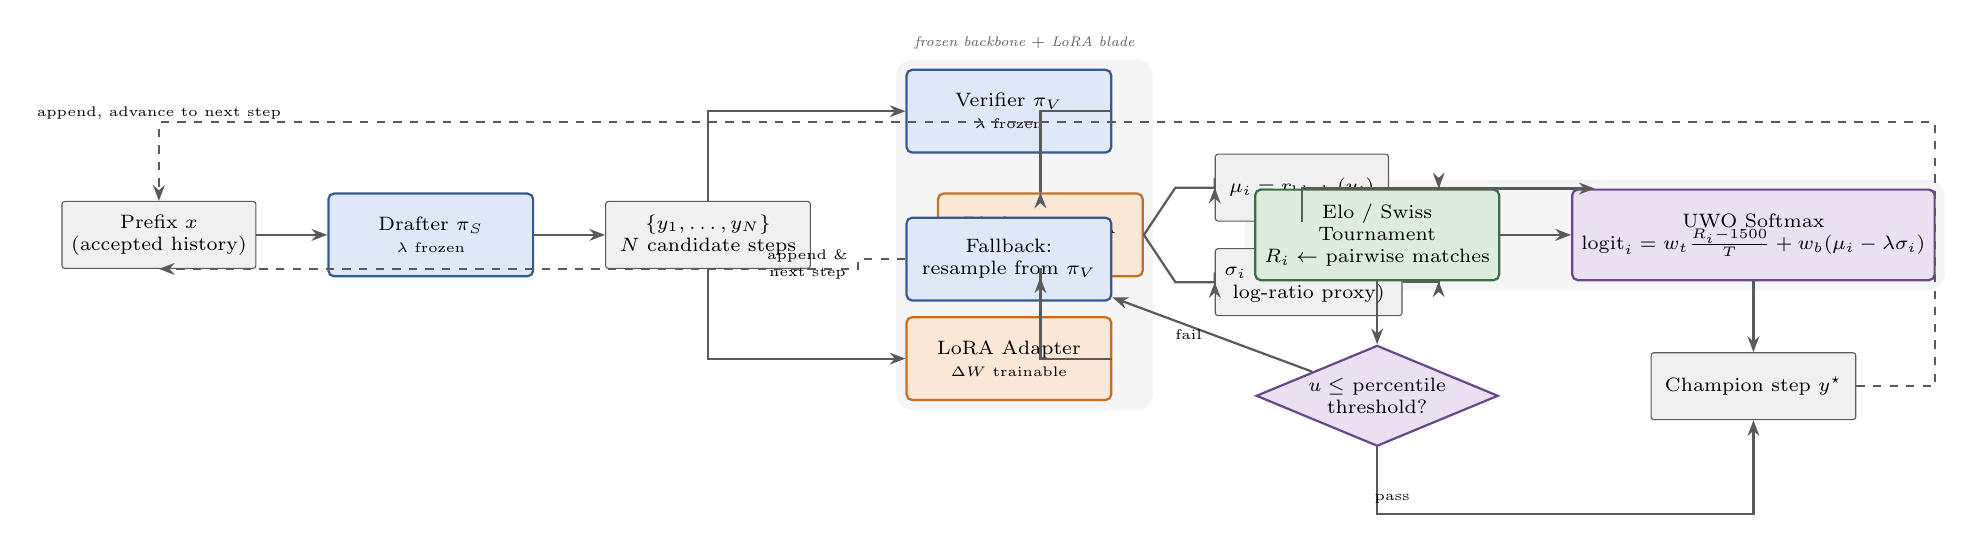
\begin{tikzpicture}[node distance=7mm and 9mm]

  % --- input ---
  \node[databox] (prefix) {Prefix $x$\\ \scriptsize(accepted history)};

  % --- drafting ---
  \node[frozenbox, right=of prefix] (drafter) {Drafter $\pi_S$\\ \tiny$\lambda$ frozen};
  \node[databox, right=of drafter, minimum width=2.6cm] (cands)
       {$\{y_1,\dots,y_N\}$\\ \scriptsize $N$ candidate steps};

  % --- scoring: verifier + LoRA blade ---
  \node[frozenbox, above right=6mm and 12mm of cands] (verifier) {Verifier $\pi_V$\\ \tiny$\lambda$ frozen};
  \node[lorabox, below right=6mm and 12mm of cands] (lora) {LoRA Adapter\\ \tiny$\Delta W$ trainable};

  \node[lorabox, right=16mm of cands, yshift=0mm] (blade)
       {Blade $\pi_{V+\mathrm{LoRA}}$\\ \scriptsize reward head};

  \node[databox, right=9mm of blade, yshift=6mm] (mu) {$\mu_i = r_{\text{blade}}(y_i)$};
  \node[databox, right=9mm of blade, yshift=-6mm] (sigma) {$\sigma_i$ (mc-dropout /\\ log-ratio proxy)};

  % --- tournament ---
  \node[tourbox, right=14mm of blade, yshift=0mm] (tour)
       {Elo / Swiss\\ Tournament\\ \scriptsize $R_i \leftarrow$ pairwise matches};

  % --- selection ---
  \node[selbox, right=9mm of tour] (uwo)
       {UWO Softmax\\ \scriptsize $\mathrm{logit}_i = w_t\frac{R_i-1500}{T} + w_b(\mu_i-\lambda\sigma_i)$};

  \node[databox, below=9mm of uwo, minimum width=2.6cm] (champ) {Champion step $y^\star$};

  % --- threshold gate ---
  \node[decision, below=8mm of tour] (gate) {$u \le$ percentile\\ threshold?};
  \node[frozenbox, below=8mm of verifier, xshift=0mm] (fallback)
       {Fallback:\\ resample from $\pi_V$};

  % ---------------- edges ----------------
  \draw[flow] (prefix) -- (drafter);
  \draw[flow] (drafter) -- (cands);
  \draw[flow] (cands.north) |- (verifier.west);
  \draw[flow] (cands.south) |- (lora.west);
  \draw[flow] (verifier.east) -| ($(blade.north)+(0,0)$) -- (blade.north);
  \draw[flow] (lora.east) -| ($(blade.south)+(0,0)$) -- (blade.south);
  \draw[flow] (blade.east) -- ++(4mm,6mm) -| (mu.west);
  \draw[flow] (blade.east) -- ++(4mm,-6mm) -| (sigma.west);
  \draw[flow] (mu.east) -| ($(tour.north)!0.5!(tour.north east)$);
  \draw[flow] (sigma.east) -| ($(tour.south)!0.5!(tour.south east)$);
  \draw[flow] (tour) -- (uwo);
  \draw[flow] (mu.south) |- ($(uwo.north west)+(3mm,0)$) node[pos=0.05]{};
  \draw[flow] (uwo) -- (champ);
  \draw[flow] (tour) -- (gate);
  \draw[flow] (gate) -- node[left, font=\tiny]{fail} (fallback);
  \draw[flow] (gate) -- ++(0,-15mm) -| node[pos=0.02, above, font=\tiny]{pass} (champ.south);
  \draw[loopflow] (fallback.west) -| ++(-6mm,0) |- (prefix.south)
        node[pos=0.28, left, font=\tiny, align=center]{append \&\\ next step};
  \draw[loopflow] (champ.east) -- ++(10mm,0) |- ($(prefix.north)+(0,10mm)$) -| (prefix.north)
        node[pos=0.55, above, font=\tiny]{append, advance to next step};

  % ---------------- grouping background ----------------
  \begin{scope}[on background layer]
    \node[groupbg, fit=(verifier)(lora)(blade), label={[font=\tiny\itshape,text=neutralgray]above:frozen backbone $+$ LoRA blade}] {};
    \node[groupbg, fit=(tour)(uwo)] {};
  \end{scope}

\end{tikzpicture}

\end{document}
